%% LyX 2.3.6.1 created this file.  For more info, see http://www.lyx.org/.
%% Do not edit unless you really know what you are doing.
\documentclass[aspectratio=169]{beamer}
\usepackage{lmodern}
\renewcommand{\sfdefault}{lmss}
\renewcommand{\ttdefault}{lmtt}
\usepackage[T1]{fontenc}
\usepackage[utf8]{inputenc}
\setlength{\parindent}{0cm}
\usepackage{array}
\usepackage{booktabs}
\usepackage{amssymb}
\usepackage{graphicx}

\makeatletter

%%%%%%%%%%%%%%%%%%%%%%%%%%%%%% LyX specific LaTeX commands.
%% Because html converters don't know tabularnewline
\providecommand{\tabularnewline}{\\}

%%%%%%%%%%%%%%%%%%%%%%%%%%%%%% Textclass specific LaTeX commands.
% this default might be overridden by plain title style
\newcommand\makebeamertitle{\frame{\maketitle}}%
% (ERT) argument for the TOC
\AtBeginDocument{%
  \let\origtableofcontents=\tableofcontents
  \def\tableofcontents{\@ifnextchar[{\origtableofcontents}{\gobbletableofcontents}}
  \def\gobbletableofcontents#1{\origtableofcontents}
}

%%%%%%%%%%%%%%%%%%%%%%%%%%%%%% User specified LaTeX commands.
%\usetheme{Warsaw}
\usetheme{Pittsburgh}
% or ...

\setbeamercovered{transparent}
% or whatever (possibly just delete it)

\setbeamertemplate{headline}{}

\definecolor{blue}{RGB}{0,102,255}
\definecolor{Babyblue}{rgb}{0.54, 0.81, 0.94}
\definecolor{mainblue}{RGB}{51, 51, 178}


\usepackage{color, colortbl}
\usepackage{xcolor}
\usepackage[utf8]{inputenc}

\usepackage{movie15}
\usepackage{animate}
\usepackage{graphicx}

\makeatother


\begin{document}
\title[BCI Framework]{EEG-based BCI monitoring framework: Real-time acquisition and visualization
from audiovisual stimulation paradigms}
\author{Yeison N. Cardona A.}
\institute{Universidad Nacional de Colombia sede Manizales\\
\medskip{}
Advisor: César Germán Castellanos Domínguez, Ph.D\\
Co-advisor: Andrés Marino Álvarez Meza, Ph.D}
\date{\today}

\makebeamertitle

%%\pgfdeclareimage[height=5cm]{assets/EscudoUN-2016.png}{assets/EscudoUN-2016.png}
%\logo{\pgfuseimage{ass}}
%\titlegraphic{
\includegraphics[width=2cm]{assets/EscudoUN-2016.png}}

%\AtBeginSection[]{\frame<beamer>{\frametitle{Outline}\tableofcontents[currentsection,currentsubsection]}}

\addtobeamertemplate{navigation symbols}{}{
	%\usebeamerfont{footline}    
	%\usebeamercolor[fg]{footline}  
	\hspace{1em} 
	\large
    {\color{mainblue}\insertframenumber/\inserttotalframenumber}
}

\let\oldcite\cite
\renewcommand*\cite[1]{{\color {gray}\tiny{\oldcite{#1}}}}

\begin{frame}{Outline}

\tableofcontents{}
\end{frame}

\section{Motivation}
\begin{frame}{BCI system}

\framesubtitle{Brain transducer}

A Brain Computer Interface (BCI) is a \textbf{hardware and software}
communication system, which enables cerebral activity alone to \textbf{control
computers or external devices} \cite{abiri2019comprehensive,nicolas-alonso_brain_2012}.

\begin{figure}
\centering{}
\includegraphics[width=0.75\textwidth]{assets/bci_system}
\end{figure}

\end{frame}
%
\begin{frame}{BCI systems}

\framesubtitle{Applications}
\begin{columns}[t]

\column{6.7cm}

\textbf{\scriptsize{}Clinical}{\scriptsize\par}
\begin{itemize}
\item {\scriptsize{}Rehabilitation \cite{mane2020bci}}{\scriptsize\par}
\item {\scriptsize{}Cognitive state analysis \cite{sophia2021real}}{\scriptsize\par}
\item {\scriptsize{}Diagnostics \cite{zolubak2019application,chepurova2022motor}}{\scriptsize\par}
\item {\scriptsize{}Assistive devices for communication, locomotion, or
movement \cite{tariq2018eeg,limchesing2021review,attallah2020bci}}{\scriptsize\par}
\end{itemize}
\textbf{\scriptsize{}Non-clinical}{\scriptsize\par}
\begin{itemize}
\item {\scriptsize{}Neuroergonomics \cite{tremmel2019estimating}}{\scriptsize\par}
\item {\scriptsize{}Smart homes \cite{maleki2021brain}}{\scriptsize\par}
\item {\scriptsize{}Neuromarketing and adversiting \cite{polat2021eeg}}{\scriptsize\par}
\item {\scriptsize{}Games \cite{vasiljevic2020brain}}{\scriptsize\par}
\item {\scriptsize{}Education \cite{taherian2018caregiver}}{\scriptsize\par}
\item {\scriptsize{}Entertainment \cite{mudgal2020brain}}{\scriptsize\par}
\item {\scriptsize{}Security and validation \cite{bansal2019eeg}}{\scriptsize\par}
\end{itemize}

\column{8cm}

The widespread use of \textbf{neurophysiological signals} to develop
BCI systems has undoubtedly varied \textbf{clinical} and\textbf{ non-clinical}
applications.

\begin{figure}
\begin{centering}
\includegraphics[width=0.35\paperwidth]{assets/uses}
\par\end{centering}
{\tiny{}}%
\noindent\begin{minipage}[t]{1\columnwidth}%
\emph{\tiny{}Left: Collection of EEG, motion capture, and EMG muscle
activity during use of a robotic exoskeleton.}{\tiny\par}

\emph{\tiny{}Right: Brain-Controlled Shark Attack!}{\tiny\par}%
\end{minipage}{\tiny\par}
\end{figure}

\end{columns}

\end{frame}
%
\begin{frame}{BCI system}

\framesubtitle{Neuroimaging methods}
\begin{columns}[t]

\column{6cm}

\textbf{\scriptsize{}Electrophysiological}{\scriptsize\par}
\begin{itemize}
\item {\scriptsize{}Electroencephalography (EEG)}{\scriptsize\par}
\item {\scriptsize{}Electroconticography (ECoG)}{\scriptsize\par}
\item {\scriptsize{}Magnetoencephalography (MEG)}{\scriptsize\par}
\end{itemize}
\textbf{\scriptsize{}Hemodynamics}{\scriptsize\par}
\begin{itemize}
\item {\scriptsize{}Funtional magnetic resonance (fMRI)}{\scriptsize\par}
\item {\scriptsize{}Near-infrared spectroscopy (NIRS)}{\scriptsize\par}
\end{itemize}

\column{8.5cm}

\noindent 
\begin{figure}
\noindent \raggedright{}\includegraphics[width=0.5\paperwidth]{notebooks/neuroimaging}
\end{figure}

\end{columns}

\textbf{\vfill{}
EEG} is the most common method  in BCI systems due to its \textbf{high
temporal resolution}, relatively \textbf{low cost}, \textbf{high portability},
and \textbf{low risks} to the users \cite{abiri2019comprehensive,nicolas-alonso_brain_2012}.

\end{frame}
%
\begin{frame}{BCI system}

\framesubtitle{Signal processing and recognition group}
\begin{columns}[t]

\column{8cm}

\begin{figure}
\begin{raggedright}
\includegraphics[width=1\textwidth]{assets/motivation_bci}
\par\end{raggedright}
{\tiny{}}%
\noindent\begin{minipage}[t]{1\columnwidth}%
\emph{\tiny{}TU Charite Campus Benjamin Franklin - Machine learning
for BCI}%
\end{minipage}{\tiny\par}
\end{figure}

The \textbf{SPGR} has interest into decoding patterns of brain activity
for the \textbf{extraction of relevant information} \cite{caicedo2021deep,collazos2020cnn}.

\column{5cm}

\begin{figure}
\raggedright{}\includegraphics[width=0.45\textheight]{assets/gcpds/gcpds-2}
\end{figure}

\end{columns}

\end{frame}

\section{Problem statement}

\begin{frame}{Problem statement}

Implementing a BCI system is an \textbf{interdisciplinary activity},
requiering knowledge about communication systems, signals acquisition,
instrumentation, clinical protocols, experiment validation, and software
development \cite{bernardi2019simplified,wolpaw2002brain}.

\begin{figure}
\centering{}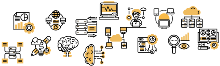
\includegraphics[width=0.75\paperwidth]{assets/interdisciplinary}
\end{figure}

\end{frame}
%
\begin{frame}{Problem statement}

\framesubtitle{Acquisition system requierements}

\textbf{Main restriction: }not all EEG acquisition systems are capable
of using BCI systems. 

\begin{figure}
\centering{}\includegraphics[width=0.7\paperwidth]{assets/embedded}
\end{figure}

There is a need to \textbf{implement a context-specific development}
to improve the base features of embedded EEG acquisition systems \cite{larocco2020systemic}.

\end{frame}
%
\begin{frame}{Problem statement}

\framesubtitle{BCI software development issues}

There is aneed for a software capable of handling BCI implementation,
but a few of them are independent, and at least \textbf{a couple is
needed to perform a complete BCI paradigm} \cite{brunner2018bci}.
\begin{columns}[t]

\column{4cm}
\begin{itemize}
\item {\scriptsize{}Behavioral sciences}{\scriptsize\par}
\item {\scriptsize{}Neuroscience}{\scriptsize\par}
\item {\scriptsize{}Psychology}{\scriptsize\par}
\item {\scriptsize{}Psychophysics}{\scriptsize\par}
\item {\scriptsize{}Linguistics}{\scriptsize\par}
\end{itemize}

\column{10cm}

\begin{figure}
\raggedright{}\includegraphics[width=0.6\paperwidth]{assets/software}
\end{figure}

\end{columns}

\end{frame}
%
\begin{frame}{Problem statement}

\framesubtitle{Computational cost}
\begin{columns}[t]

\column{7cm}

\textbf{\scriptsize{}}{\scriptsize\par}

\textbf{\scriptsize{}Close-loop BCI system}{\scriptsize\par}
\begin{itemize}
\item {\scriptsize{}Data acquisition}{\scriptsize\par}
\item {\scriptsize{}Signals database/storage}{\scriptsize\par}
\item {\scriptsize{}Feature processing (extraction and classification)}{\scriptsize\par}
\item {\scriptsize{}Visualization (temporal, spatial and frequency domain)}{\scriptsize\par}
\item {\scriptsize{}Command generation for actuators}{\scriptsize\par}
\item {\scriptsize{}Command database}{\scriptsize\par}
\item {\scriptsize{}Feedback acquisition}{\scriptsize\par}
\end{itemize}

\column{7.3cm}

It is necesary to distribute this task in order to \textbf{reduce
the computing complexity }of a BCI, \textbf{increasing the reliability
}of the overall system performance \cite{sugiarto2009application}.

\begin{figure}
\centering{}\includegraphics[width=0.4\paperwidth]{assets/feduc-06-782969-g001}
\end{figure}

\end{columns}

\vfill{}
Centralized systems are susceptible to \textbf{slowdowns} due to unexpected
processing costs \cite{assran2020advances,deshmukh2021collaborative}.
\end{frame}

\section{State-of-the-art BCI systems}
\begin{frame}{State-of-the-art BCI systems}


\framesubtitle{Embedded acquisition systems for BCI}
\begin{center}
{\tiny{}}%
\begin{tabular}{>{\raggedright}m{2.8cm}>{\raggedright}m{2.2cm}>{\raggedright}m{1.2cm}>{\raggedright}m{1.7cm}>{\raggedright}m{2cm}>{\raggedright}m{1.8cm}}
\toprule 
\textbf{\tiny{}BCI hardware} & \textbf{\tiny{}Electrode types} & \textbf{\tiny{}\# Channels} & \textbf{\tiny{}Protocol} & \textbf{\tiny{}Sampling rate} & \textbf{\tiny{}Open hardware}\tabularnewline
\midrule
\textbf{\tiny{}q.DSI 10/20} & {\tiny{}Flexible / Dry} & {\tiny{}21} & {\tiny{}BLE} & {\tiny{}250 Hz - 900 Hz} & {\tiny{}No}\tabularnewline
\textbf{\tiny{}InteraXon Inc. Muse} & {\tiny{}Rigid / Dry} & {\tiny{}5} & {\tiny{}BLE} & {\tiny{}220 Hz} & {\tiny{}No}\tabularnewline
\textbf{\tiny{}Emotive EPOC+} & {\tiny{}Rigid / Wet} & {\tiny{}14} & {\tiny{}RF} & {\tiny{}128 Hz} & {\tiny{}No}\tabularnewline
\textbf{\tiny{}Biosemi ActiveTwo} & {\tiny{}Flexible / Wet} & {\tiny{}256} & {\tiny{}USB} & {\tiny{}2 KHz - 16 KHz} & {\tiny{}No}\tabularnewline
\textbf{\tiny{}actiCAP slim/snap} & {\tiny{}Flexible / Wet / Dry} & {\tiny{}16} & {\tiny{}USB} & {\tiny{}2 KHz - 20 KHz} & {\tiny{}No}\tabularnewline
\textbf{\tiny{}NeuroSky Mind Wave} & {\tiny{}Rigid / Dry} & {\tiny{}1} & {\tiny{}RF} & {\tiny{}250 Hz} & {\tiny{}No}\tabularnewline
\textbf{\tiny{}\cellcolor{Babyblue}OpenBCI} & \textbf{\tiny{}\cellcolor{Babyblue}}{\tiny{}Flexible / Wet / Dry} & \textbf{\tiny{}\cellcolor{Babyblue}}{\tiny{}8, 16} & \textbf{\tiny{}\cellcolor{Babyblue}}{\tiny{}RF/BLE/Wi-Fi} & \textbf{\tiny{}\cellcolor{Babyblue}}{\tiny{}250 Hz - 16 KHz} & \textbf{\tiny{}\cellcolor{Babyblue}}{\tiny{}Yes}\tabularnewline
\end{tabular}{\tiny\par}
\par\end{center}

\vfill{}

\textbf{Licensing} is a key feature for hardware inclusion in a \textbf{real
BCI environments}. Solutions that includes \textbf{open components}
can increase the \textbf{technology acceptance} and \textbf{wide spreading}
\cite{duan2021educational,legenvre2020open,powell2012democratizing}.
\end{frame}
%
\begin{frame}{State-of-the-art BCI systems}

\framesubtitle{OpenBCI}
\begin{center}
{\tiny{}}%
\begin{tabular}{>{\raggedright}m{3.5cm}>{\raggedright}m{1.3cm}>{\raggedright}m{1.5cm}>{\raggedright}m{1.5cm}>{\raggedright}m{2cm}>{\raggedright}m{2cm}}
\toprule 
\textbf{\tiny{}OpenBCI Cyton} & \textbf{\tiny{}\# Channels} & \textbf{\tiny{}Digital inputs} & \textbf{\tiny{}Analog inputs} & \textbf{\tiny{}Max sample rate} & \textbf{\tiny{}Featured protocol}\tabularnewline
\midrule
\textbf{\tiny{}RFduino} & {\tiny{}8} & {\tiny{}5} & {\tiny{}3} & {\tiny{}250 Hz} & {\tiny{}Serial}\tabularnewline
\addlinespace[-0.1cm]
\textbf{\tiny{}RFduino + Daisy} & {\tiny{}16} & {\tiny{}5} & {\tiny{}3} & {\tiny{}250 Hz} & {\tiny{}Serial}\tabularnewline
\addlinespace[-0.1cm]
\textbf{\tiny{}RFduino + Wi-Fi shield} & {\tiny{}8} & {\tiny{}2} & {\tiny{}1} & {\tiny{}16 KHz} & {\tiny{}TCP (over Wi-Fi)}\tabularnewline
\addlinespace[-0.1cm]
\textbf{\tiny{}RFduino + Wi-Fi shield + Daisy} & {\tiny{}16} & {\tiny{}2} & {\tiny{}1} & {\tiny{}8 KHz} & {\tiny{}TCP (over Wi-Fi)}\tabularnewline
\addlinespace[-0.1cm]
\end{tabular}{\tiny\par}
\par\end{center}
\begin{columns}[t]

\column{5.5cm}

\begin{figure}
\raggedright{}\includegraphics[width=0.4\paperwidth]{assets/OpenBCI-board-overview-26}
\end{figure}


\column{7cm}

\bigskip{}
\bigskip{}
\bigskip{}
\textbf{OpenBCI} is the \textbf{most flexible} and \textbf{featured}
acquisition board for \textbf{electrophysiological signals} \cite{laport2019comparative,kuhn2021performance,yohanandan2018robust,knierim2021open}.
\end{columns}

\end{frame}
%
\begin{frame}{State-of-the-art BCI systems}

\framesubtitle{BCI software}
\begin{center}
{\tiny{}}%
\begin{tabular}{>{\raggedright}m{4cm}>{\raggedright}m{1.5cm}>{\raggedright}m{1.2cm}>{\raggedright}m{1.45cm}>{\raggedright}m{1.1cm}>{\raggedright}m{1cm}>{\raggedright}m{1cm}}
\toprule 
\textbf{\tiny{}BCI software} & \textbf{\tiny{}Stimuli delivery} & \textbf{\tiny{}Devices} & \textbf{\tiny{}Data analysis} & \textbf{\tiny{}Close-loop} & \textbf{\tiny{}Extensibility} & \textbf{\tiny{}License}\tabularnewline
\midrule
\textbf{\tiny{}\cellcolor{Babyblue}BCI2000} & \textbf{\tiny{}\cellcolor{Babyblue}}{\tiny{}Yes} & \textbf{\tiny{}\cellcolor{Babyblue}}{\tiny{}A large set} & \textbf{\tiny{}\cellcolor{Babyblue}}{\tiny{}In software} & \textbf{\tiny{}\cellcolor{Babyblue}}{\tiny{}Yes} & \textbf{\tiny{}\cellcolor{Babyblue}}{\tiny{}Yes} & \textbf{\tiny{}\cellcolor{Babyblue}}{\tiny{}GPL}\tabularnewline
\textbf{\tiny{}\cellcolor{Babyblue}OpenViBE} & \textbf{\tiny{}\cellcolor{Babyblue}}{\tiny{}Yes} & \textbf{\tiny{}\cellcolor{Babyblue}}{\tiny{}A large set} & \textbf{\tiny{}\cellcolor{Babyblue}}{\tiny{}In software} & \textbf{\tiny{}\cellcolor{Babyblue}}{\tiny{}Yes} & \textbf{\tiny{}\cellcolor{Babyblue}}{\tiny{}Yes} & \textbf{\tiny{}\cellcolor{Babyblue}}{\tiny{}AGPL-3}\tabularnewline
\textbf{\tiny{}Neurobehavioral Systems Presentation} & {\tiny{}Yes} & {\tiny{}Official list} & {\tiny{}In software} & {\tiny{}Yes} & {\tiny{}Yes} & {\tiny{}Proprietary}\tabularnewline
\textbf{\tiny{}EEGLAB} & {\tiny{}No} & {\tiny{}Matlab} & {\tiny{}System Matlab} & {\tiny{}No} & {\tiny{}-} & {\tiny{}Proprietary}\tabularnewline
\textbf{\tiny{}PsychoPy} & {\tiny{}Yes} & {\tiny{}NO} & {\tiny{}NO} & {\tiny{}No} & {\tiny{}Yes} & {\tiny{}GPL}\tabularnewline
\textbf{\tiny{}Millisecond Inquisit Lab} & {\tiny{}Yes} & {\tiny{}Serial} & {\tiny{}NO} & {\tiny{}No} & {\tiny{}No} & {\tiny{}Proprietary}\tabularnewline
\textbf{\tiny{}\cellcolor{Babyblue}OpenBCI} & \textbf{\tiny{}\cellcolor{Babyblue}}{\tiny{}No} & \textbf{\tiny{}\cellcolor{Babyblue}}{\tiny{}Proprietary} & \textbf{\tiny{}\cellcolor{Babyblue}}{\tiny{}No} & \textbf{\tiny{}\cellcolor{Babyblue}}{\tiny{}No} & \textbf{\tiny{}\cellcolor{Babyblue}}{\tiny{}Yes} & \textbf{\tiny{}\cellcolor{Babyblue}}{\tiny{}MIT}\tabularnewline
\end{tabular}{\tiny\par}
\par\end{center}
\begin{columns}[t]

\column{8cm}

\textbf{Specialized laboratory equipment} is necessary to calculate
latencies and make corrections\textbf{ offline} \cite{appelhoff2021we,razavi2022opensync}.

\column{6cm}

Some systems are able to creating \textbf{control signals} and performing
corrections in \textbf{real-time} \cite{davis2020stimulus}.
\end{columns}

\end{frame}
%
\begin{frame}{State-of-the-art BCI systems}

\framesubtitle{Real-time and computational cost handling}
\begin{columns}[t]

\column{6.5cm}

\textbf{Offline}
\begin{itemize}
\item Cloud-based strategies \cite{abe2021neuroscience}.
\item Cost Vs. Accuracy \cite{al2018accuracy,ahmadi2012brain}.
\end{itemize}

\column{7cm}

\begin{figure}
\begin{raggedright}
\animategraphics[autoplay,loop,width=2.5in]{6}{assets/p300/p300-}{0}{44}
\par\end{raggedright}
\raggedright{}{\tiny{}}%
\noindent\begin{minipage}[t]{1\columnwidth}%
\textcolor{black}{\emph{\tiny{}Cognionics Dry EEG P300 Speller Demo}}%
\end{minipage}{\tiny\par}
\end{figure}

\end{columns}

\textbf{Real-time}
\begin{itemize}
\item Real-time and parallel learning\cite{netzer2020real,hasan2020computationally}.
\item Stimuli delivery precision and standarization \cite{amaducci2019rthybrid,muniz2009rtbiomanager}.
\item Large neural data streams has become workable thanks to microprocessors,
and specialized open-source software \cite{potter2014closed}.\vfill{}
\end{itemize}
\end{frame}
%
\begin{frame}{Question research}

How to develop an independent \textbf{EEG-based BCI monitoring framework}
that merges \textbf{real-time acquisition}, \textbf{visualization}
from audiovisual stimulation paradigms, and an \textbf{integrated
development environment }using \textbf{OpenBCI}? 
\end{frame}

\section{Aims}
\begin{frame}{General aim}
To develop an \textbf{EEG-based} BCI monitoring \textbf{framework}
with \textbf{real-time acquisition and visualization} for audiovisual
stimulation paradigms using \textbf{OpenBCI}, focused on designing,
performing, and validating BCI systems to conduct experiments in the
stages of design and testing.

\end{frame}
%
\begin{frame}{Specific aims}
\begin{itemize}
\item To implement a cross-platform library for \textbf{OpenBCI} hardware
that allows distributed functionalities, \textbf{low-level board configurations},
an \textbf{acquisition protocol}, \textbf{data storage}, and external
\textbf{inputs handler.} 
\item To implement a \textbf{distributed computing} paradigm that allows
managing acquisition boards, acquiring EEG signals through a network,
\textbf{synchronizing markers}, \textbf{measuring latencies}, and
\textbf{delivering stimuli experiments }into a \textbf{decentralized
environment} using a\textbf{ SBC}\footnote{\textbf{SBC: }Single Board Computing}
scheme.
\item To develop an independent interface with an\textbf{ IDE}\footnote{\textbf{IDE: }Integrated Development Environment}\textbf{
}featured to configure the \textbf{acquisition system}, design \textbf{real-time}
visualizations, and perform \textbf{stimuli delivery}.
\end{itemize}
\end{frame}

\section{Development}
\begin{frame}{Development {[}obj1{]}}

\framesubtitle{High-level acquisition driver for OpenBCI}

\begin{figure}
\includegraphics[width=0.75\paperwidth]{assets/drivers}
\end{figure}

\textbf{Device-first} drivers development that allows specific configurations
\textbf{enhance capabilities} and the \textbf{integration} with computational
devices.
\end{frame}
%
\begin{frame}{Development {[}obj1{]}}

\framesubtitle{Hight-level features}

\vspace{-1.3cm}

\begin{columns}[t]
\hspace{-1.5cm}

\column{7cm}

\begin{figure}
\includegraphics[height=0.45\textheight]{assets/bad_markers_autodetection}
\end{figure}


\column{4.5cm}

\begin{figure}
\centering{}\animategraphics[autoplay,loop,width=6cm]{10}{assets/marker_sync/marker_sync-}{001}{482}
\end{figure}

\end{columns}

\vfill{}
\textbf{OpenBCI-Stream}\footnote{https://openbci-stream.readthedocs.io}
consists of a high-level drivers for Cyton boards with \textbf{context-specific
preprocessing task} like \textbf{markers synchronization} and \textbf{'BAD'
trials dropping}.
\end{frame}
%
\begin{frame}{Development {[}obj1{]}}

\framesubtitle{Drivers comparison}
\begin{center}
{\tiny{}}%
\begin{tabular}{>{\raggedright}p{2.5cm}>{\raggedright}p{2.5cm}>{\raggedright}p{2.5cm}>{\raggedright}p{2.5cm}>{\raggedright}p{2.5cm}}
\toprule 
\textbf{\tiny{}Feature} & \textbf{\tiny{}OpenBCI Python (2015) and pyOpenBCI (2015)} & \textbf{\tiny{}OpenBCI LSL (2017)} & \textbf{\tiny{}BrainFlow (2018)} & \textbf{\tiny{}\cellcolor{Babyblue}OpenBCI Stream (2020)}\tabularnewline
\midrule
\textbf{\tiny{}Acquisition boards} & {\tiny{}All OpenBCI boards} & {\tiny{}All OpenBCI boards} & {\tiny{}+10 different boards} & \textbf{\tiny{}\cellcolor{Babyblue}OpenBCI Cyton}\tabularnewline
\textbf{\tiny{}Distributed paradigm} & {\tiny{}No} & {\tiny{}No} & {\tiny{}No} & \textbf{\tiny{}\cellcolor{Babyblue}Yes}\tabularnewline
\textbf{\tiny{}Impedance measurement} & {\tiny{}No} & {\tiny{}No} & {\tiny{}No} & \textbf{\tiny{}\cellcolor{Babyblue}Yes}\tabularnewline
\textbf{\tiny{}Set boardmodes} & {\tiny{}No} & {\tiny{}No} & {\tiny{}No} & \textbf{\tiny{}\cellcolor{Babyblue}Yes}\tabularnewline
\textbf{\tiny{}Set sampling rate} & {\tiny{}No} & {\tiny{}No} & {\tiny{}No} & \textbf{\tiny{}\cellcolor{Babyblue}Yes}\tabularnewline
\textbf{\tiny{}Set package size} & {\tiny{}No} & {\tiny{}No} & {\tiny{}No} & \textbf{\tiny{}\cellcolor{Babyblue}Yes}\tabularnewline
\textbf{\tiny{}Markers syncronization} & {\tiny{}No} & {\tiny{}No} & {\tiny{}No} & \textbf{\tiny{}\cellcolor{Babyblue}Yes}\tabularnewline
\textbf{\tiny{}Asynchronous acquisition} & {\tiny{}No} & {\tiny{}Yes} & {\tiny{}No} & \textbf{\tiny{}\cellcolor{Babyblue}Yes}\tabularnewline
\textbf{\tiny{}Data storage} & {\tiny{}No} & {\tiny{}No} & {\tiny{}Yes} & \textbf{\tiny{}\cellcolor{Babyblue}Yes}\tabularnewline
\textbf{\tiny{}Active development} & {\tiny{}No} & {\tiny{}No} & {\tiny{}Yes} & \textbf{\tiny{}\cellcolor{Babyblue}Yes}\tabularnewline
\bottomrule
\end{tabular}{\tiny\par}
\par\end{center}

\end{frame}
%
\begin{frame}{Development {[}obj2{]}}

\framesubtitle{Real-time and distributed implementation}

\begin{figure}
\includegraphics[width=0.9\paperwidth]{assets/latencies2}
\end{figure}

\textbf{Real-time} guarantees that all data blocks of duration $P$
will be \textbf{available} to the user in a time lower than $P$,
\textbf{regardless of the block duration}. 
\end{frame}
%
\begin{frame}{Development {[}obj2{]}}

\framesubtitle{Latency comparison}
\begin{center}
{\tiny{}}%
\begin{tabular}{>{\raggedright}p{3cm}>{\raggedright}p{1.3cm}>{\raggedright}p{1.3cm}>{\raggedright}p{1.3cm}>{\raggedright}p{1.5cm}>{\raggedright}p{1.3cm}>{\raggedright}p{1.3cm}}
\toprule 
\textbf{\tiny{}BCI system} & \textbf{\tiny{}Sample rate} & \textbf{\tiny{}Block size} & \textbf{\tiny{}Jitter} & \textbf{\tiny{}Communication} & \textbf{\tiny{}Distributed} & \textbf{\tiny{}Latency}\tabularnewline
\midrule
\textbf{\tiny{}BCI2000 + DT3003} & {\tiny{}160 Hz} & {\tiny{}6.35 ms} & {\tiny{}0.67 ms} & {\tiny{}Wired} & {\tiny{}No} & \textbf{\tiny{}51.9 \%}\tabularnewline
\textbf{\tiny{}BCI2000 + NI6024 E} & {\tiny{}25 kHz} & {\tiny{}40 ms} & {\tiny{}0.75 ms} & {\tiny{}Wired} & {\tiny{}No} & \textbf{\tiny{}27.5 \%}\tabularnewline
\textbf{\tiny{}BCI2000 + g.USBamp} & {\tiny{}1200 Hz} & {\tiny{}83.3 ms} & {\tiny{}5.91 ms} & {\tiny{}Wired} & {\tiny{}No} & \textbf{\tiny{}14, 30, 48 \%}\tabularnewline
\textbf{\tiny{}OpenViBE + TMSi Porti32} & {\tiny{}512 Hz} & {\tiny{}62.5 ms} & {\tiny{}3.07 ms} & {\tiny{}Optical MUX} & {\tiny{}No} & \textbf{\tiny{}100.4 \%}\tabularnewline
\textbf{\tiny{}\cellcolor{Babyblue}BCI-Framework} & \textbf{\tiny{}\cellcolor{Babyblue}1000 Hz} & \textbf{\tiny{}\cellcolor{Babyblue}100 ms} & \textbf{\tiny{}\cellcolor{Babyblue}5.7 ms} & \textbf{\tiny{}\cellcolor{Babyblue}Wireless} & \textbf{\tiny{}\cellcolor{Babyblue}Yes} & \textbf{\tiny{}\cellcolor{Babyblue}56 \% (fixed)}\tabularnewline
\bottomrule
\end{tabular}{\tiny\par}
\par\end{center}

\textbf{BCI implementations} \textbf{performance} can be mesaured
through all close-loop process, the \textbf{latency} and the \textbf{jitter}
describe the relation of the acquisition system with the \textbf{command
generation}.
\end{frame}
%
\begin{frame}{Development {[}obj3{]}}

\framesubtitle{The connection support multiple hardware configurations and electrodes
montages}

\begin{figure}
\centering{}\animategraphics[autoplay,loop,width=5in]{10}{assets/bci_framework_connect2/animation-}{000}{579}
\end{figure}

\end{frame}
%
\begin{frame}{Development {[}obj3{]}}

\framesubtitle{The integrated development environment includes previsualization
and debugging}

\begin{figure}
\centering{}\animategraphics[autoplay,loop,width=5in]{10}{assets/bci_framework_ide2/animation-}{000}{365}
\end{figure}

\end{frame}
%
\begin{frame}{Development {[}obj3{]}}

\framesubtitle{The stimuli delivery}

\begin{figure}
\centering{}\animategraphics[autoplay,loop,width=5in]{10}{assets/bci_framework_delivery2/animation-}{000}{611}
\end{figure}

\end{frame}
%
\begin{frame}{Development {[}obj3{]}}

\framesubtitle{BCI-Framework: Real-time analysis}

\begin{figure}
\centering{}\animategraphics[autoplay,loop,width=5in]{10}{assets/bci_framework_plot2/animation-}{000}{274}
\end{figure}

\end{frame}

\section{Demostration}
\begin{frame}{Demostration}
\begin{center}
OpenBCI Stream\footnote{https://openbci-stream.readthedocs.io} +
BCI Framework\footnote{https://docs.bciframework.org}
\par\end{center}
\end{frame}

\section{Conclusions and academic discussion}
\begin{frame}{Conclusions}

\begin{description}
\item [{Obj1}] A \textbf{brand-new} set of drivers was developed with the
ability to take advantage of the hardware and all the benefits of
the \textbf{ADS1299}. In addition, a unique feature has been included
to \textbf{synchronize markers} using the low-level characteristics
of the acquisition board.
\item [{Obj2}] All the components needed to achieve a \textbf{flexible},
\textbf{scalable}, and \textbf{comprehensive BCI system} were identified,
into a framework that integrates a \textbf{fully-featured environment}
with almost all the tools to develop complete \textbf{research-grade
BCI systems}.
\item [{Obj3}] Although it is a distributed system, \textbf{real-time streaming
is guaranteed}, \textbf{latency and jitter are kept within accepted
ranges for closed-loop} BCI systems, and acquisition methodology ensures
that the \textbf{bad sampling data can be labeled and processed accordingly}.
\end{description}
\end{frame}
%
\begin{frame}{Future work}

\framesubtitle{Custom acquisition system and validation}
\begin{itemize}
\item Although the selected board for this work, OpenBCI Cyton, is one of
the best performing and configurable hardware, \textbf{a new acquisition
board that integrates the latest technology and communication protocols
on a single board is needed}. i.e. only the \textbf{ADS1299} in combination
with an \textbf{ESP32} can provide many usable features in BCI.
\item Although the system has been proven under specific applications and
some databases have been generated, \textbf{further integration and
validation with the methodologies developed by the SPGR are needed}.
\end{itemize}

\end{frame}
%
\begin{frame}{Academic discussion}

\framesubtitle{Papers, patents and software registers}
\begin{itemize}
\item {[}2022{]} Paper submitted to \emph{SoftwareX - Journals | Elsevier}
with the name \textbf{\textquotedbl A real-time acquisition, visualization,
and stimuli delivery Python-based tool for neurophysiological experiments\textquotedbl}\emph{.}
\item {[}2022{]} The systems were submitted to the \textbf{Crearlo no es
suficiente} summons for a \emph{patentability search process} with
the \emph{Universidad Nacional de Colombia sede Manizales} as main
beneficiary with the title \textbf{\textquotedbl MÉTODO Y SISTEMA
PARA LA SINCRONIZACIÓN DE MARCADORES ASOCIADOS A SISTEMAS DE INTERFAZ
CEREBRO-COMPUTADOR\textquotedbl}, postulation \emph{ID 343 }and
Application number \emph{NC2022/0007405} from May 28, 2022.
\item {[}2022{]} A script developed with BCI-Framework for\textbf{ Motor
imagery paradigm with game-based stimulus (Pacman interface)} was
submitted to the software register in the \emph{Universidad Nacional
de Colombia sede Manizales}.
\end{itemize}
\end{frame}

\section{Acknowledgements}
\begin{frame}{Acknowledgements}

This research would not have been possible without the support provided
by the project \emph{Caracterización Morfológica de Estructuras Cerebrales
por Técnicas de Imagen para el Tratamiento Mediante Implantación Quirúrgica
de Neuroestimuladores en la Enfermedad de Parkinson (código 110180763808)}
funded by \textbf{MINCIENCIAS}.
\end{frame}

\section{References}
\begin{frame}[allowframebreaks]{References}

{\tiny{}\bibliographystyle{apalike}
\bibliography{references}
}{\tiny\par}

\end{frame}

\end{document}
